\chapter{Markov Equivalence}


%----------------------------------------------------------------------------------------
%	Markov Equivalence
%----------------------------------------------------------------------------------------

\section{Goal}

\null \quad \quad In order to reduce the cost of a query on a graph $G$, we will exploit the observation that two Bayesian networks with distinguishable structures can model the same probability distribution. In this case, the corresponding graphs are called \textit{Markov equivalent}. Given a query on a graph $G$, we search for a Markov equivalent graph $G'$ such that the cost of the query is minimized when considered on $G'$ instead of $G$.  \newline
\null \quad \quad To do so, we must develop a robust understanding of Markov equivalence. This includes: how to identify whether two graphs are Markov equivalent, how a graph can be altered while remaining in the set of Markov equivalent graphs (called the \textit{Markov equivalence class}), and how computations of queries on a graph are altered when the graph structure is altered. \newline
\null \quad \quad In this chapter, we present definitions, theorems, and examples to establish a sufficient understanding of Markov equivalence for this purpose. 

\section{Basic Properties of Markov Equivalence}

\begin{definition}[Markov equivalence~\cite{verma}]
Two directed acyclic graphs $G$ and $G'$ are \textbf{Markov equivalent} if for every Bayesian network $B = (G, \theta_{G})$, there exists a Bayesian network $B' = (G', \theta_{G'})$ such that $B$ and $B'$ describe the same probability distribution, and vice versa. This is denoted $G \ME G'$.
\end{definition}
\newpage

\begin{definition}[Markov equivalence class~\cite{verma}]
The set of all DAGs which are Markov equivalent to a DAG $G$ is called the \textbf{Markov equivalence class}(MEC) of $G$, denoted $[G]$.
\end{definition}

\null \quad \quad Significant research has been done to characterize Markov equivalence classes (~\cite{chickering, verma, andersson}). This research has identified several key features of a graphs which allow us to more easily identify reversible edges and construct MECs. The following definitions outline several properties of graphs (and edges within them) which we will use to determine whether two graphs lie in the same MEC. Furthermore, it will help us build an understanding of how a graph can be manipulated without altering which MEC it belongs to. 


%----------------------covered defn
\begin{definition}[Covered Edge~\cite{chickering}]\label{defcoverededge} 
Given a DAG $G=(V,E)$, an edge $e = (X, Y) \in E$ is called \textbf{covered} in $G$ iff $\prod\nolimits_{Y}^{G} = \prod\nolimits_{X}^{G} \cup \ X$. That is, $(X, Y)$ is covered in $G$ iff $X$ and $Y$ have identical parents in $G$ with the exception that $X$ is not a parent of itself.
\end{definition}

\begin{center}
\begin{figure}[h!]
\centering
\begin{tikzpicture}
\Vertex[size=.5, color=gray]{x1}
\Vertex[x = 2, size=.5, color=white]{x2}
\Vertex[y = -2, ,size=.5,color=white]{x3}
\Vertex[y=-2, x=2 ,size=.5,color=white]{x4}
\Edge[Direct, distance=0.5, color=red](x1)(x2)
\Edge[Direct, distance=0.5, color=red](x2)(x4)
\Edge[Direct, distance=0.5](x4)(x3)
\Edge[Direct, distance=0.5](x1)(x4)
\end{tikzpicture}
\caption{ }
\label{fig:covedge}
\end{figure}
\end{center}

In Figure~\ref{fig:covedge}, for example, the red edges are the only covered edges; the upper edge is covered because its vertices both have no parents; the righthand edge is covered because its vertices share the gray vertex as their single parent. 

%----------------------\covered defn


%----------------------skeleton defn

\begin{definition} [Skeleton]
Let $G=(V,E)$ be a directed graph. The undirected graph $G' = (V, E')$ which is constructed by removing the orientation of all edges in $E$ is called the \textbf{skeleton} of $G$. 
\end{definition}
 
\begin{center}
\begin{tikzpicture}
\Vertex[size=.5, color=white]{x1}
\Vertex[x = 2, size=.5, color=white]{x2}
\Vertex[y = -2, ,size=.5,color=white]{x3}
\Vertex[y=-2, x=2 ,size=.5,color=white]{x4}
\Edge[Direct, distance=0.5](x1)(x2)
\Edge[Direct, distance=0.5](x1)(x2)
\Edge[Direct, distance=0.5](x1)(x4)
\Edge[Direct, distance=0.5](x2)(x4)
\Edge[Direct, distance=0.5](x4)(x3)
\Text[x=1, y= -3]{$G$}

\scalebox{1.5}{
\Text[x=2.5 ,y=-.6667]{$\implies$} %because of scalebox: y = 1/1.5, x=3.75/1.5
}

\Vertex[x=5.5, size=.5, color=white]{x1b}
\Vertex[x=7.5, size=.5, color=white]{x2b}
\Vertex[x=5.5, y = -2, ,size=.5,color=white]{x3b}
\Vertex[x=7.5, y=-2,size=.5,color=white]{x4b}
\Edge[distance=0.5](x1b)(x2b)
\Edge[distance=0.5](x1b)(x2b)
\Edge[distance=0.5](x1b)(x4b)
\Edge[distance=0.5](x2b)(x4b)
\Edge[distance=0.5](x3b)(x4b)
\Text[x=6.5, y= -3]{$G' =\ $ skeleton$(G)$}
\end{tikzpicture}
\end{center}


%----------------------\skeletion defn 

%----------------------v-structures defn
\begin{definition} [v-structure]
A set of three vertices $X, Y, Z$ of a graph $G = (V,E)$ is called a \textbf{v-structure} (or immorality) iff  $(X, Y) \in E$ and $ (Z, Y) \in E$ but $X$ and $Z$ are not adjacent.
 
\begin{center}
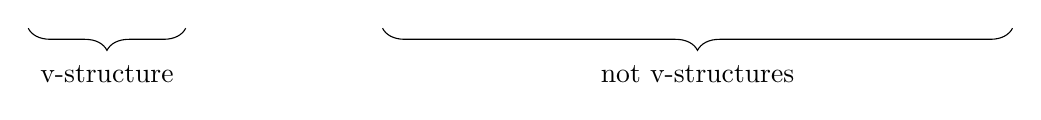
\begin{tikzpicture}
\Vertex[x=-4.5, size=.5, color=white]{x1}
\Vertex[x = -2.5, size=.5, color=white]{x2}
\Vertex[y = -1.5, x=-3.5 ,size=.5,color=white]{x3}
\Edge[Direct, distance=0.5](x1)(x3)
\Edge[Direct, distance=0.5](x2)(x3)

\Vertex[size=.5, color=white]{x1}
\Vertex[x = 2, size=.5, color=white]{x2}
\Vertex[y = -1.5, x=1 ,size=.5,color=white]{x3}
\Edge[Direct, distance=0.5](x1)(x3)
\Edge[Direct, distance=0.5](x3)(x2)

\Vertex[x = 3,size=.5, color=white]{x1}
\Vertex[x = 5, size=.5, color=white]{x2}
\Vertex[y = -1.5, x=4, size=.5,color=white]{x3}
\Edge[Direct, distance=0.5](x3)(x1)
\Edge[Direct, distance=0.5](x3)(x2)

\Vertex[x = 6,size=.5, color=white]{x1}
\Vertex[x = 8, size=.5, color=white]{x2}
\Vertex[y = -1.5, x=7, size=.5,color=white]{x3}
\Edge[Direct, distance=0.5](x1)(x2)
\Edge[Direct, distance=0.5](x2)(x3)
\Edge[Direct, distance=0.5](x1)(x3)


\draw [decorate,decoration={brace,amplitude=8pt,mirror,raise=-5ex}]
  (-4.5,-3) -- (-2.5,-3) node[midway,yshift=.5em]{v-structure};
\draw [decorate,decoration={brace,amplitude=8pt,mirror,raise=-5ex}]
  (0,-3) -- (8,-3) node[midway,yshift=.5em]{not v-structures};
\end{tikzpicture}
\end{center}

\end{definition}
%----------------------\v-structures defn


\begin{lemma}[Criterion for Markov equivalence~\cite{verma}]\label{meccriterion} %verma theorem 1, pearl 1989 paper. 
Two graphs are equivalent iff they have the same skeleton and v-structures. 
\end{lemma}

\begin{proof}
A sketch of the proof is provided, as the complete proof involves many definitions and details which are not presented in this paper. First, we use the definition of an \textbf{active route} (sometimes called active path) with respect to a set $\mathbb{Z}$: a route $[X_{0}, X_{1}, ... X_{n}]$ in which all nodes $X_{i}$ are themselves \textbf{active}, meaning that (1) every middle node of a v-structure with respect to $\mathcal{Z}$ either is or has a descendant in $\mathcal{Z}$, and (2) every other node in the route is outside $\mathcal{Z}$. \newline
\null \quad \quad The proof depends on two lemmas presented in the same paper: \textbf{Lemma 1} has the consequence that adjacency of nodes is invariant among equivalent DAGs. \textbf{Lemma 2} has the consequence that one can determine the presence or absence of v-structures by observing certain separation properties of the graph alone, and vice versa. 
The two lemmas are unified with an inductive step to show that active paths in one DAG correspond to active paths in a Markov equivalent DAG. Furthermore, properties of active paths allow us to conclude that the DAGs must have the same skeleton and v-structures. 
\end{proof}

%----------------------\reversible edge defn
\begin{definition}[Irreversible edge~\cite{andersson}]
Let $G$ be a DAG. A directed edge $(X,Y) \in G$ is called \textbf{irreversible} in $G$ if changing $(X,Y)$ to $(Y,X)$ either creates or destroys a v-structure, or creates a directed cycle. An edge which is not irreversible is called \textbf{reversible}. 
\end{definition}
%----------------------\reversible edge defn

\begin{lemma}[Covered edges are exactly reversible edges~\cite{chickering}]\label{coveredrev} %lemma 1 in chickering
Let $G = (V,E)$ be a DAG, let $X,Y \in V$ and let $e = (X, Y) \in E$. Let $G' = (V,E')$ be the DAG constructed from $G$ by reversing the edge $(X, Y)$ to $(Y, X)$. Then $G$ and $G'$ are equivalent iff $e$ is a covered edge in $G$.
\end{lemma}

\begin{proof}
Let $G = (V,E)$ be a DAG. A sketch of the proof is as follows (see ~\cite{chickering} for the full proof):
	\begin{myindentpar}{1em}
	(\textbf{if}) Suppose $e = (X,Y)$ is a covered edge in $G$. Let $G'$ be equivalent to $G$, except that $e$ is reveresed to $e' = (Y,X)$. Then:
		\begin{itemize}
		\item $G'$ is also a DAG. To show this, suppose that $G'$ is not a DAG. Since $G$ and $G'$ only differ by $e' = (Y,X)$, there must be a directed cycle including $e'$ in $G'$. Then there is a path in $G$ from $Y$ to $X$. By assumption, $Y$ and $X$ have a shared set of parents. However, one can conclude from this that $G$ also contains a cycle because every cycle must include at least one node from $\prod\nolimits_{X}^{G}$, and therefore is not a DAG, a contradiction. By this contradiction, we conclude that $G'$ must be a DAG. 
		\item $G' \ME G$. Firstly, $G$ and $G'$ trivially have the same skeleton, since they only differ by the orientation of edge $e$. Then, if they were \textit{not} Markov equivalent graphs, they would differ by a v-structure. If $G'$ has a v-structure not present in $G$, it must include the edge $(Y,X)$. However, this would imply that $X$ has a parent which is not a neighbor to $Y$, contradicting the assumption that $e$ is covered. A similar argument holds for the scenario where $G$ has a v-structure not present in $G'$. 
		\end{itemize}
	
	(\textbf{only if}) We now show that if $e=(X,Y)$ is not a covered edge in $G$, we are in one of two cases: either $G'$ contains a directed cycle, or $G'$ is a DAG which is not equivalent to $G$. If $(X,Y)$ is not a covered edge in $G$, then at least one of the following hold:
	\begin{enumerate}
		\item There is a node $Z \neq X$ which is a parent of $Y$ but not of $X$. 
		\item There s a node $W$ which is a parent of $X$ but not of $Y$. 
	\end{enumerate}
	Let $Z \neq X$ be a parent of $Y$ in $G$ but not a parent of $X$ in $G$. If $Z$ and $X$ are not neighbors, then there is a v-structure consisting of edges $(X,Y)$ and $(Y,Z)$ in $G$ which does not exist in $G'$. If $X$ is a parent of $Z$ in $G$, then it must also be a parents of $Z$ in $G'$, which would imply that $G'$ contains a directed cycle and is therefore not a DAG. \newline
	\null \quad \quad The argument for the second case is equivalent, assuming $W$ is a parent of $X$ in $G$ and deriving a v-structure with $(W,X)$ and $(X,Y)$ which exists in $G'$ but not $G$. We conclude that $G$ would have to contain a directed cycle. In both scenarios, we have derived a contradiction which shows that $(X,Y)$ must be covered in $G$. \qedhere


\end{myindentpar}
\end{proof}


%------------------------------------------MEC threenode example
\begin{example}[Members of Markov equivalence class~\cite{verma}]\label{mecexample}
Consider the four DAGs in Figure~\ref{fig:sameMECseparateMEC}.

\begin{figure}[h!]
\begin{center}
\begin{tikzpicture}
\Vertex[x = 0, y=3, size=.5, color=white, label=$X$]{x}
\Vertex[x = 0, y=1.5, size=.5, color=white, label=$Y$]{y}
\Vertex[x=0, y = 0, size=.5,color=white, label=$Z$]{z}
\Edge[Direct, distance=0.5](x)(y)
\Edge[Direct, distance=0.5](y)(z)
\Text[x=-.8 ,y=3]{$G_{1}$}

\Vertex[x = 6, y=3, size=.5, color=white, label=$X$]{x}
\Vertex[x = 6, y=1.5, size=.5, color=white, label=$Y$]{y}
\Vertex[x=6, y = 0, size=.5,color=white, label=$Z$]{z}
\Edge[Direct, distance=0.5](z)(y)
\Edge[Direct, distance=0.5](y)(x)
\Text[x=5.2 ,y=3]{$G_{3}$}

\Vertex[x = 2, y=.8, size=.5, color=white, label=$X$]{x}
\Vertex[x = 4, y=.8, size=.5, color=white, label=$Z$]{z}
\Vertex[x=3, y = 2.2, size=.5,color=white, label=$Y$]{y}
\Edge[Direct, distance=0.5](y)(x)
\Edge[Direct, distance=0.5](y)(z)
\Text[x=2.1 ,y=1.8]{$G_{2}$}

\Vertex[x = 9, y=2.2, size=.5, color=white, label=$X$]{x}
\Vertex[x = 11, y=2.2, size=.5, color=white, label=$Z$]{z}
\Vertex[x=10, y = .8, size=.5,color=white, label=$Y$]{y}
\Edge[Direct, distance=0.5](x)(y)
\Edge[Direct, distance=0.5](z)(y)
\Text[x=9.1 ,y=1.25]{$G_{4}$}

\draw [decorate,decoration={brace,amplitude=8pt,mirror,raise=-5ex}]
  (-.8,-1.3) -- (6.8,-1.3) node[midway,yshift=.5em]{same MEC};
\draw [decorate,decoration={brace,amplitude=8pt,mirror,raise=-5ex}]
  (9,-1.3) -- (11,-1.3) node[midway,yshift=.5em]{separate MEC};
\end{tikzpicture}
\end{center}
\caption{}
\label{fig:sameMECseparateMEC}
\end{figure}

\null \quad \quad The fact that $G_{1}, G_{2}$, and $G_{3}$ are in the same MEC while $G_{4}$ is not can be seen by considering the joint probability distribution $p(X,Y,Z)$ of each of the graphs. 

\begin{myindentpar}{3em}
\begin{spacing}{1.25}
	$G_{1}$ : \quad $p(X,Y,Z) = p(X) \cdot p(Y|X) \cdot p(Z|Y)$ \newline
	$G_{2}$ : \quad $p(X,Y,Z) = p(Y) \cdot p(X|Y) \cdot p(Z|Y)$ \newline
	$G_{3}$ : \quad $p(X,Y,Z) = p(Z) \cdot p(Y|Z) \cdot p(X|Y)$
	\end{spacing}
\end{myindentpar}
By Bayes' theorem, all of the values of $G_{2}$ can be completely determined from values from $G_{1}$:
	$$
	p(X)p(Y|X) = p(X,Y) = p(Y)p(X|Y)
	$$
and $p(Z|Y)$ is unchanged. A similar application of Bayes' theorem shows that $G_{3}$ is completely determined by $G_{1}$ and $G_{2}$:
	$$
	p(z) \cdot p(Y|Z) = p(Z,Y) = p(Y) \cdot p(Z|Y)
	$$
where $p(Y)$ can be attained directly from $G_{2}$ and $p(Z|Y)$ can be attained from $G_{1}$. Therefore, we can conclude that since all three describe the same distribution, they lie in the same equivalence class. In contrast, the joint probability for $G_{4}$ is given by
	$$
	p(X,Y,Z) = p(X) \cdot p(Z) \cdot p(Y|X,Z)
	$$
which can not be determined from the values of $G_{1}, G_{2}$ and $G_{3}$. This is because in [$G_{1}$] %(but not in $G_{2}$ and $G_{3}$), 
$X$ is conditionally independent from $Y$ and $Z$, that is, $X$ is only independent in the circumstance that we are given values for $Y$ and $Z$. Meanwhile, in $G_{4}$, $X$ is marginally independent of $Z$, that is, independent in the circumstance that we ignore $Y$. Conditional independence does not provide information about marginal independence, and conversely, marginal independence does not imply conditional independence. Therefore, $G_{4}$ describes a different distribution, and does not lie in [$G_{1}$]. 

\end{example}
%------------------------------------------MEC threenode example


\begin{corollary}\label{coveredMEC}~\cref{meccriterion} and ~\cref{coveredrev} together imply that the graph $G'$ which results from only reversing the orientation of a covered edge $(X, Y) \in G$ is in the MEC of $[G]$. 
\begin{proof}
This follows from the fact that edge reversal does not change the skeleton of the graph $G$ (since no edges are added nor removed) and reversing covered edges does not alter the v-structures of $G$ (\cref{coveredrev}), thus the v-structures and skeleton are unchanged. 
\end{proof}
\end{corollary}



%----------------------------------------------------------------------------------------
%	Effects of Edge Reversal
%----------------------------------------------------------------------------------------
\section{Effects of Edge Reversal}


%---------------------------------------------- two node example

\begin{lemma}
Given a single directed edge between two parentless nodes in which the joint probability $p(X_{1},X_{2}) = p(X_{1}) \cdot p(X_{2}|X_{1})$, the new factorization of the joint probability distribution $p(X_{1},X_{2})$ can be computed as follows using only the known quantities $p(X_{1})$ and $p(X_{2}|X_{1})$:
$$
p(X_{1}, X_{2})\ \ = \ \ \sum_{X_{1}} p(X_{2}|X_{1}) \cdot p(X_{1}) \frac{ p(X_{2}|X_{1}) \cdot p(X_{1}) }{ \sum_{X_{1}} p(X_{2}|X_{1}) \cdot p(X_{1})}.
$$
\end{lemma}

\begin{figure}[h!]
\begin{center}
\begin{tikzpicture}
\Vertex[size=1, color=white, label=$X_{1}$]{x1}
\Vertex[x=4,size=1,color=white, label=$X_{2}$]{x2}
\Edge[Direct](x1)(x2)
\end{tikzpicture}

\scalebox{1.2}{$\Big\Downarrow$} 

\begin{tikzpicture}
\Vertex[size=1, color=white, label=$X_{1}$]{x1}
\Vertex[x=4,size=1,color=white, label=$X_{2}$]{x2}
\Edge[Direct](x2)(x1)
\end{tikzpicture}
\end{center}
\caption{}
\end{figure}

\begin{proof}
This follows directly from Bayes' theorem, which gives us
\begin{align*} 
	p(X_{1}| X_{2})	& \ \ = \ \ \frac{p(X_{2}|X_{1}) \cdot p(X_{1})}{p(X_{2})}	\\[2em]
				& \ \ = \ \ \frac{p(X_{2}|X_{1}) \cdot p(X_{1})}{\sum_{X_{1}} p(X_{2}|X_{1}) \cdot p(X_{1})}. 
\end{align*}
\end{proof}
%---------------------------------------------- \two node example


%---------------------------------------------- shared parent lemma

\begin{lemma}\label{sharedparent}
Given a directed edge between two vertices $X_{1}$ and $X_{2}$ with a shared parent vertex $X_{P}$, the joint probability $p(X_{1}, X_{2}, X_{p})$ after switching edge $(X_{1}, X_{2})$ to $(X_{2},X_{1})$ can be computed as follows using only known quantities $p(X_{p})$,  $p(X_{1}|X_{p})$, and \newline $p(X_{2}|X_{1},X_{p})$:
\begin{align*}
	p(X_{1},X_{2},X_{P}) & \ \ = \ \ 	[\frac{   p(X_{2}|X_{1},X_{p}) \cdot p(X_{1}|X_{p})   }{  \sum_{X_{1}} p(X_{1}|X_{p})\cdot p(X_{2}|X_{1},X_{p})  }  ] \\[1em] 
				& \quad \quad  \cdot [\sum_{X_{1}} p(X_{1}|X_{p})\cdot p(X_{2}|X_{1},X_{p})] \cdot p(X_{p}).
\end{align*}
\end{lemma}


\begin{figure}[h!]
\begin{center}
\begin{minipage}[t]{0.35\textwidth}
\begin{center}
\begin{tikzpicture}
\Vertex[x = 2, size=1, color=white, label=$X_{P}$]{xP}
\Vertex[x=4, y=-3,size=1,color=white, label=$X_{1}$]{x1}
\Vertex[x=0, y=-3,size=1,color=white, label=$X_{2}$]{x2}
\Edge[Direct, distance=0.5](x1)(x2)
\Edge[Direct, distance=0.5](xP)(x2)
\Edge[Direct, distance=0.5](xP)(x1)
\end{tikzpicture}
\end{center}
\end{minipage}
~
\begin{minipage}[t]{0.1\textwidth}
\begin{center}
\vspace{-7em}
\scalebox{1.5}{$\implies$} 
\end{center}
\end{minipage}
~
\begin{minipage}[t]{0.35\textwidth}
\begin{center}
\begin{tikzpicture}
\Vertex[x = 2, size=1, color=white, label=$X_{P}$]{xP}
\Vertex[x=4, y=-3,size=1,color=white, label=$X_{1}$]{x1}
\Vertex[x=0, y=-3,size=1,color=white, label=$X_{2}$]{x2}
\Edge[Direct, distance=0.5](x2)(x1)
\Edge[Direct, distance=0.5](xP)(x2)
\Edge[Direct, distance=0.5](xP)(x1)
\end{tikzpicture}
\end{center}
\end{minipage}
\end{center}
\caption{}
\end{figure}

	%---------------------------------------------- generalization of shared parent lemma
	
\begin{remark}
Furthermore, because this result does not depend on $p(X_{p})$, we can conclude that for a set of shared parents $P = \{X_{P_{1}},X_{P_{2}},\ ...\ X_{P_{i}}\}$ of two nodes $X_{1}$ and $X_{2}$, the same equality holds. Additionally, note that any reversal of an edge with a set of shared parents is MEC-invariant, since all such edges are covered (~\cref{coveredMEC}).
\end{remark}

\begin{figure}[h!]
\begin{center}
\begin{tikzpicture}
\Vertex[x = -1, size=1, color=white, label=$X_{P_{1}}$]{xP1}
\Vertex[x = .5, size=1, color=white, label=$X_{P_{2}}$]{xP2}
\Vertex[x = 5, size=1, color=white, label=$X_{P_{i}}$]{xPi}

\Text[y=.15, x=2.75]{$\textbf{   .\ \    .\ \    .  }$}

\Vertex[x=4, y=-3,size=1,color=white, label=$X_{1}$]{x1}
\Vertex[x=0, y=-3,size=1,color=white, label=$X_{2}$]{x2}

\Edge[Direct, distance=0.5](x2)(x1)

\Edge[Direct, distance=0.5](xP1)(x2)
\Edge[Direct, distance=0.5](xP1)(x1)

\Edge[Direct, distance=0.5](xP2)(x2)
\Edge[Direct, distance=0.5](xP2)(x1)

\Edge[Direct, distance=0.5](xPi)(x2)
\Edge[Direct, distance=0.5](xPi)(x1)
\end{tikzpicture}
\end{center}
\caption{}
\end{figure}
	
	%----------------------------------------------\generalization of shared parent lemma


\begin{proof}
From before the edge reversal, we have access to the values $p(X_{p}), p(X_{1}|X_{p})$, and $p(X_{2}|X_{1},X_{p})$. Our goal is to determine the new joint probability distribution $p(X_{1}, X_{2}, X_{p})$ using this information. Therefore, we must find $p(X_{p}), p(X_{2}|X_{p})$, and $p(X_{1}|X_{2},X_{p})$. First, $p(X_{p})$ is already trivially available. Then, to compute $p(X_{1}|X_{2},X_{p})$,

\begin{align*}
p(X_{1}|X_{2},X_{p}) & \ \ = \ \  \frac{ p(X_{1}, X_{2}, X_{p})  }{ p(X_{2},X_{p})  } \\[1em]
			    & \ \ = \ \  \frac{ p(X_{2}|X_{1},X_{p}) \cdot p(X_{1},X_{p}) }{ p(X_{2},X_{p}) } \\[1em]
			    & \ \ = \ \  \frac{ p(X_{2}|X_{1},X_{p}) \cdot p(X_{1}|X_{p}) \cdot p(X_{p}) }{ p(X_{2}|X_{1},X_{p}) } \\[1em]
			    & \ \ = \ \  \frac{ p(X_{2}|X_{1},X_{p}) \cdot p(X_{1}|X_{p}) }{ p(X_{2}|X_{p}) }
\end{align*}

which depends only on known quantities once we compute

\begin{align*}
p(X_{2}|X_{p}) 	& \ \ = \ \ \frac{p(X_{2},X_{p})}{p(X_{p})} \\[1em]
			& \ \ = \ \ \frac{1}{p(X_{p})} \sum_{X_{1}} p(X_{1},X_{2},X_{p}) \\[1em]
			& \ \ = \ \ \frac{1}{p(X_{p})} \sum_{X_{1}} p(X_{1},X_{p}) \cdot \frac{p(X_{2},X_{1}, X_{p})}{p(X_{1},X_{p})} \\[1em]
			& \ \ = \ \ \sum_{X_{1}} p(X_{1}|X_{p}) \cdot p(X_{2}|X_{1},X_{p}).
\end{align*}

Together, these give us 
\begin{align*}
p(X_{1},X_{2},X_{p})	& \ \ = \ \ p(X_{1}|X_{2},X_{p}) \cdot p(X_{2}|X_{p}) \cdot  p(X_{p}) \\[1em]
				& \ \ = \ \    
				[\frac{   p(X_{2}|X_{1},X_{p}) \cdot p(X_{1}|X_{p})   }{  \sum_{X_{1}} p(X_{1}|X_{p}) \cdot p(X_{2}|X_{1},X_{p})  }  ] \\[1em] 
				&  \quad \quad \cdot [\sum_{X_{1}} p(X_{1}|X_{p})\cdot p(X_{2}|X_{1},X_{p})] \cdot p(X_{p}).
\end{align*}
\end{proof}

\begin{remark}
Notice that the above cancels to show that the two graphs are Markov equivalent, since $p(X_{1}|X_{2},X_{p}) \cdot p(X_{2}|X_{p}) \cdot p(X_{p})=  p(X_{2}|X_{1},X_{p}) \cdot p(X_{1}|X_{p}) \cdot p(X_{p}).$
\end{remark}

%---------------------------------------------- \shared parent lemma



%----------------------------------------------------------------------------------------
%	Find Reversible Edges of a DAG Model
%----------------------------------------------------------------------------------------
\section{Identifying Reversible Edges}


\begin{definition}[Essential edge~\cite{andersson},~\cite{flesch}] %definition 10 flesch, definition 2.1 Andersson
An \textbf{essential edge} (also called a compelled edge~\cite{chickering}) of a graph $G = (V,E)$ is an edge $(X,Y) = e \in E$ such that for every graph $G' = (V,E')$ in $[G]$, the orientation of $e \in E$ is unchanged. That is, there is no graph $G' = (V,E')$ in $[G]$ such that $(Y,X) \in E'.$
\end{definition}

% ---------------------essential graph defn
\begin{definition} [Essential graph~\cite{andersson}]
The \textbf{essential graph} of a Markov equivalence class $[G]$ is a mixed graph $G_{*}$ such that the only directed edges in $G_{*}$ are essential edges of $[G]$. That is,
\begin{itemize}
	\item The directed edge $ e = (X, Y) \in G_{*}$ iff  $e \in G$ for every graph $G \in [G]$,
	\item The undirected edge ${X,Y} \in G_{*}$ iff there are graphs $G_{1}$ and $G_{2} \in [G]$ such that $(X, Y)$ in $G_{1}$ and $(Y, X)$ in $G_{2}$. 
\end{itemize}
\end{definition}
% --------------------\-essential graph defn


% ---------------------essential graph example
\begin{example}\label{essentialgraphexample} In this example, we identify the essential edges of a Markov equivalence class and construct the essential graph. Consider the following DAG $G = (V,E)$:

\begin{figure}[h!]
\begin{center}
\begin{tikzpicture}
\Vertex[x = 2, y=0, size=.5, color=white, label=$Y$]{y}
\Vertex[x = 4, y=0, size=.5, color=white, label=$Z$]{z}
\Vertex[x=3, y = 1.4, size=.5,color=white, label=$X$]{x}
\Edge[Direct, distance=0.5](x)(y)
\Edge[Direct, distance=0.5](y)(z)
\Edge[Direct, distance=0.5](x)(z)
\Text[x=3 ,y=-.5]{$G$}
\end{tikzpicture}
\end{center}
\caption{}
\end{figure}

We use the following realizations to show that the graph has no essential edges. If we switch any edge in $G$, the resulting graph $G'$ becomes one of two cases:
\begin{itemize}
	\item $G'$ is cyclic, and therefore no longer a DAG, meaning this edge was irreversible. 
		\newline \null \quad Example: reversing edge $(X,Z)$ as in \textbf{(A)} creates a cycle.

		\begin{center}
		\begin{tikzpicture}
		
			\Vertex[x = 1, y=0, size=.5, color=white, label=$Y$]{y}
			\Vertex[x = 3, y=0, size=.5, color=white, label=$Z$]{z}
			\Vertex[x=2, y = 1.4, size=.5,color=white, label=$X$]{x}
			\Edge[Direct, distance=0.5](x)(y)
			\Edge[Direct, distance=0.5](y)(z)
			\Edge[Direct, distance=0.5](z)(x)
			\Text[x=2 ,y=-1]{\textbf{(A)}}

		\end{tikzpicture}
		\end{center} 
			
	\item $G'$ is equivalent to $G$ up to relabeling, and therefore in the same MEC.
		\newline \null \quad Example: reversing $(X,Y)$ and changing labels according to $X \rightarrow Y',\  Y\rightarrow Z',$  and $Z \rightarrow X'$, as in \textbf{(B)}.
\end{itemize} 

\begin{center}
\begin{tikzpicture}

\Vertex[x = 6, y=0, size=.5, color=white, label=$Y$]{y}
\Vertex[x = 8, y=0, size=.5, color=white, label=$Z$]{z}
\Vertex[x=7, y = 1.4, size=.5,color=white, label=$X$]{x}
\Edge[Direct, distance=0.5](y)(x)
\Edge[Direct, distance=0.5](y)(z)
\Edge[Direct, distance=0.5](x)(z)

\Text[x=9 ,y=-1]{\textbf{(B)}}
\Text[x=9 ,y=.7]{\large $\implies$}
\Text[x=9 ,y=1.2]{relabeling}

\Vertex[x = 10, y=0, size=.5, color=white, label=$Z'$]{z'}
\Vertex[x = 12, y=0, size=.5, color=white, label=$X'$]{x'}
\Vertex[x=11, y = 1.4, size=.5,color=white, label=$Y'$]{y'}
\Edge[Direct, distance=0.5](y')(z')
\Edge[Direct, distance=0.5](z')(x')
\Edge[Direct, distance=0.5](y')(x')
\end{tikzpicture}
\end{center}

Thus the following graphs are included in [$G$], though they are not the entire MEC. The red edges in each are those with orientation which differs from edges in $G$. Notice, however, that some relabeling was required, meaning these edges do not necessarily correspond (under this new labeling) to covered edges.

\begin{center}
\begin{tikzpicture}
\Vertex[x = 2, y=0, size=.5, color=white, label=$Y'$]{y}
\Vertex[x = 4, y=0, size=.5, color=white, label=$Z'$]{z}
\Vertex[x=3, y = 1.4, size=.5,color=white, label=$X'$]{x}
\Edge[Direct, distance=0.5, color=red](y)(x)
\Edge[Direct, distance=0.5](y)(z)
\Edge[Direct, distance=0.5](x)(z)
\Text[x=3 ,y=-.5]{$G'_{1}$}

\Vertex[x = 6, y=0, size=.5, color=white, label=$Y'$]{y}
\Vertex[x = 8, y=0, size=.5, color=white, label=$Z'$]{z}
\Vertex[x=7, y = 1.4, size=.5,color=white, label=$X'$]{x}
\Edge[Direct, distance=0.5, color=red](z)(x)
\Edge[Direct, distance=0.5](y)(z)
\Edge[Direct, distance=0.5, color=red](y)(x)
\Text[x=7 ,y=-.5]{$G'_{2}$}

\Vertex[x = 10, y=0, size=.5, color=white, label=$Y'$]{y}
\Vertex[x = 12, y=0, size=.5, color=white, label=$Z'$]{z}
\Vertex[x=11, y = 1.4, size=.5,color=white, label=$X'$]{x}
\Edge[Direct, distance=0.5](x)(z)
\Edge[Direct, distance=0.5, color=red](z)(y)
\Edge[Direct, distance=0.5](x)(y)
\Text[x=11 ,y=-.5]{$G'_{3}$}
\end{tikzpicture}
\end{center}

Therefore, under some circumstance, for every edge $(U,V) = e \in G$, there is a DAG $G' \in [G]$ such that $(V,U) \in G'$. This means that $G$ has no essential edges. We construct the essential graph $G_{*}$ of $G$ by removing the orientation of all non-essential edges in $G$: 

\begin{center}
\begin{tikzpicture}
\Vertex[x = 6, y=0, size=.5, color=white, label=$Y$]{y}
\Vertex[x = 8, y=0, size=.5, color=white, label=$Z$]{z}
\Vertex[x=7, y = 1.4, size=.5,color=white, label=$X$]{x}
\Edge[Direct, distance=0.5](x)(y)
\Edge[Direct, distance=0.5](y)(z)
\Edge[Direct, distance=0.5](x)(z)
\Text[x=7 ,y=-.5]{$G$}
\Text[x=9 ,y=.7]{\large $\implies$}


\Vertex[x = 10, y=0, size=.5, color=white, label=$Z'$]{y}
\Vertex[x = 12, y=0, size=.5, color=white, label=$X'$]{z}
\Vertex[x=11, y = 1.4, size=.5,color=white, label=$Y'$]{x}
\Edge[distance=0.5](x)(y)
\Edge[distance=0.5](y)(z)
\Edge[distance=0.5](x)(z)
\Text[x=11 ,y=-.5]{$G_{*}$}
\end{tikzpicture}
\end{center}

\end{example}

% ---------------------\essential graph example


\begin{remark}
Andersson et. al.~\cite{andersson} demonstrate that essential graphs are consistent across a MEC and unique to it, meaning an essential graph can be used as a representative for a given MEC. Furthermore, essential graphs are not necessarily DAGs, and therefore do not generally belong to the MEC that they represent. \newline
\null \quad \quad This can be seen by the fact that the distinction between two MECs lies entirely in either differences in their skeletons or in the orientations of their compelled edges. \newline

\textit{``It is only in the heart that one can see rightly; what is essential is invisible to the eye.'' -Antoine de Saint-Exupéry, The Little Prince.}
\end{remark}


%--------------------\essential vs covered edge disctinction example
\begin{remark}
One should take care to note the distinction between implications about non-essential edges versus covered edges: 
\begin{itemize}
	\item For $G = (V,E)$, an edge $e \in E$ is non-essential iff there exists a graph $G'$ in $[G]$ such that $e$ is reversed,
	\item An edge $e$ in $G$ is covered iff the graph $G'$ derived from \textit{only} reversing $e$, is in the MEC of $G$. (Follows from ~\cref{coveredMEC}.)
\end{itemize}
That is, reversing $e$ \textit{exclusively} while remaining in the MEC of $G$ requires $e$ to be covered. Meanwhile, a non-essential edge $e \in G$ may require other edges in $G$ to be reversed as well to remain in the same MEC. This means that not all non-essential edges can be reversed at a given time. The following example demonstrates that some configurations of non-essential edge reversals are not possible if we wish to remain in the MEC of $G$.
\end{remark}

\begin{example}
Again consider members of the Markov equivalence class seen in ~\cref{mecexample}. The positions of the nodes are visually rearranged for clarity, but no properties are changed. \newline
\begin{figure}[h!]
\begin{center}
\begin{tikzpicture}
\Vertex[x = 0, y=3, size=.5, color=white, label=$X$]{x}
\Vertex[x = 0, y=1.5, size=.5, color=white, label=$Y$]{y}
\Vertex[x=0, y = 0, size=.5,color=white, label=$Z$]{z}
\Edge[Direct, distance=0.5](x)(y)
\Edge[Direct, distance=0.5](y)(z)
\Text[x=-.8 ,y=3]{$G_{1}$}

\Vertex[x = 3, y=3, size=.5, color=white, label=$X$]{x}
\Vertex[x = 3, y=1.5, size=.5, color=white, label=$Y$]{y}
\Vertex[x=3, y = 0, size=.5,color=white, label=$Z$]{z}
\Edge[Direct, distance=0.5](y)(x)
\Edge[Direct, distance=0.5](y)(z)
\Text[x=2.2 ,y=3]{$G_{2}$}

\Vertex[x = 6, y=3, size=.5, color=white, label=$X$]{x}
\Vertex[x = 6, y=1.5, size=.5, color=white, label=$Y$]{y}
\Vertex[x=6, y = 0, size=.5,color=white, label=$Z$]{z}
\Edge[Direct, distance=0.5](z)(y)
\Edge[Direct, distance=0.5](y)(x)
\Text[x=5.2 ,y=3]{$G_{3}$}

\Vertex[x = 10, y=3, size=.5, color=white, label=$X$]{x}
\Vertex[x = 10, y=1.5, size=.5, color=white, label=$Y$]{y}
\Vertex[x=10, y = 0, size=.5,color=white, label=$Z$]{z}
\Edge[Direct, distance=0.5](z)(y)
\Edge[Direct, distance=0.5](x)(y)
\Text[x=9.2 ,y=3]{$G_{4}$}

\draw [decorate,decoration={brace,amplitude=8pt,mirror,raise=-5ex}]
  (-.8,-1.3) -- (6.8,-1.3) node[midway,yshift=.5em]{same MEC};
\draw [decorate,decoration={brace,amplitude=8pt,mirror,raise=-5ex}]
  (9,-1.3) -- (11,-1.3) node[midway,yshift=.5em]{separate MEC};
\end{tikzpicture}
\end{center}
\caption{}
\end{figure}
\null \quad \quad Notice that edge $(Y,Z) \in$  $G_{1}$ is non-essential, since there exists another graph (namely $G_{3}$) in  [$G_{1}$] such that $(Z,Y) \in$ $G_{3}$. Therefore, we know that there exists some combination of edge reversals such that $(Y,Z)$ can be reversed without leaving [$G_{1}$]. However, if we choose to switch only $(Y,Z)$ to $(Z,Y)$, we have exactly graph $G_{4}$, which is no longer in the same MEC. Therefore, the fact that an edge is non-essential does not provide information about the circumstances in which the edge can be reversed without altering the MEC; only that in some context, it can be. This realization leads us to ~\cref{essentialsubset}.
\end{example}
%--------------------\essential vs covered edge distinction example

%--------------------covered is subset of essential
\begin{corollary}\label{essentialsubset}
Let $E_{c}$ be the set of covered edges in $G$, and let $E_{e}$ be the set of essential edges in $G$. Then $E_{c} \subseteq \bar{E_{e}}$, the set of non-essential edges in $G$.
\begin{proof}
This follows directly from the realization that non-essential edges can be switched while remaining in the same MEC under the correct conditions, while covered edges can be switched immediately, without regard to other edge conditions (the conditions for their reversal are always met). 
\end{proof}
\end{corollary}

\begin{example}
We use the graph $G$ from Example \ref{essentialgraphexample} to demonstrate Corollary \ref{essentialsubset}. Of course, this is not sufficient for a proof, but rather helps to contextualize the lemma. 

\begin{figure}[h!]
\begin{center}
\begin{tikzpicture}
\Vertex[x = 2, y=0, size=.5, color=white, label=$Y$]{y}
\Vertex[x = 4, y=0, size=.5, color=white, label=$Z$]{z}
\Vertex[x=3, y = 1.4, size=.5,color=white, label=$X$]{x}
\Edge[Direct, distance=0.5](x)(y)
\Edge[Direct, distance=0.5](y)(z)
\Edge[Direct, distance=0.5](x)(z)
\Text[x=3 ,y=-.5]{$G$}
\end{tikzpicture}
\end{center}
\caption{}
\end{figure}

 In~\cref{essentialgraphexample} we determined that all edges $e_{i} \in E$ of $G=(V,E)$ are non-essential, so the set of non-essential edges $E_{G}^{N} = \{(X,Y), (Y,Z), (X,Z) \}$. We can quickly see that the only covered edge of $G$ is $(Y,Z)$ since $Y$ and $Z$ share a single parent $X$, not including $Z$ itself. Then, indeed, $\{(Y,Z) \} \subset E_{G}^{N}$.

\end{example}
%--------------------\covered is subset of essential


% ---------------------reversible edge conceptions
\begin{remark} There are two scenarios we consider for finding reversible edges, that is, edges which can be reversed without altering the MEC of the graph:
\begin{itemize} 
\item Firstly, we may wish to find the set of edges which can be immediately reversed in one step, without regard to other edges in the graph. This coincides with the set of covered edges. 
\item Secondly, we may wish to find the set of edges which can ever be reversed within a graph, under the correct conditions of other edges being reversed beforehand/simultaneously. This coincides with the set of non-essential edges.
 \end{itemize}
\end{remark}
% --------------------\-reversible edge conceptions

%---------------------essential vs covered edge diagram
\begin{figure}[h!]
\begin{center}
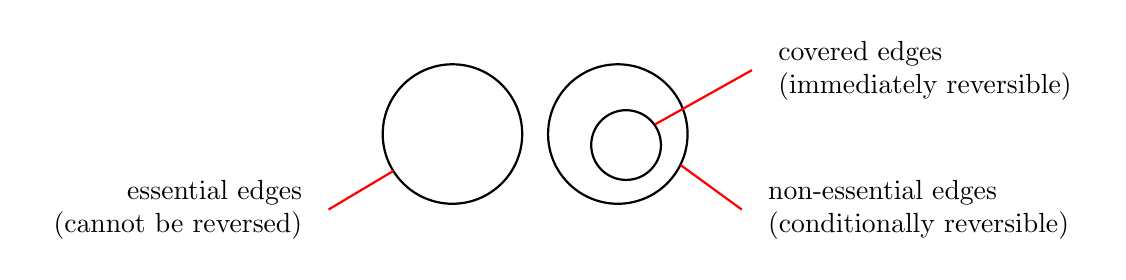
\begin{tikzpicture}[scale=0.7]
	\draw[thick] (1cm,0) circle (36pt);
	\draw[thick] (4,0) circle (36pt);
	\draw[thick] (4.15,-.2) circle (18pt);
	
	\draw[red, thick] (1cm+-30.4pt,-19pt)--(1cm+-64pt,-39pt);
	\draw[red, thick] (4cm + 32.4pt,-16pt)--(4cm+64pt,-39pt);
	\draw[red, thick] (4.15cm + 15pt, 5pt)--(4.15cm+65, 33pt);
	
	\node [left] at (1cm+-64pt, -39pt) {\begin{tabular}{r} essential edges \\ (cannot be reversed) \end{tabular}};
	\node [right] at (4cm+64pt, -39pt) {\begin{tabular}{l} non-essential edges \\ (conditionally reversible) \end{tabular}};
	\node [right] at (4.15cm+65, 33pt) {\begin{tabular}{l} covered edges \\ (immediately reversible) \end{tabular}};
\end{tikzpicture}
\end{center}
\caption{}
\end{figure}

%---------------------\essential vs covered edge diagram






\begin{theorem}[Edge reversal sequence.~\cite{chickering}]\label{reversalsequence}
Given two Markov equivalent DAGs $G$ and $G'$, there exists a sequence of distinct edge reversals in $G$ with the following properties:
\begin{itemize}
	\item Each edge reversed in $G$ is a covered edge,
	\item After each reversal, $G$ is a DAG and $G \ME G'$
	\item After all reversals, $G = G'$. 
\end{itemize}
That is, we can transform $G$ into $G'$ via a finite sequence of covered edge reversals, such that all of the intermittently resulting graphs $G_{1}, G_{2},...G_{n} \ME G, G'$. 
\end{theorem}

\begin{proof}
Chickering's ~\cite{chickering} proof defines the procedure \textbf{Procedure Find-Edge} which takes a DAG $G$ as input. At each step, the procedure identifies a next edge to reverse. To be reversible, such an edge must be covered, by \cref{coveredrev}. The proof demonstrates that such an edge is identifiable when $G$ and $G'$ remain unequal, and each reversal reduces the number of edges in total which must be reversed, eventually transforming $G$ into $G'$. 
\end{proof}

%---------------------\Algorithm for finding covered edges






%%%%%%%%%POSSIBLE THINGS TO ADD BELOW%%%%%%%%%%%%%%%%%%%



%----------------------------------------------------------------------------------------
%	Constructing the Essential Graph of a DAG Model
%----------------------------------------------------------------------------------------
%\section{Essential Graph of a DAG Model}
%
%We quickly see that construction of the essential graph $G_{*}$ of a DAG model $G$ is quite complicated, as it involves identifying all essential edges of $G$, which in turn involves having access to or a characterization of all DAGs in the MEC $[G]$. Andersson et. al.~\cite{andersson} have done significant work to characterize all DAGs which lie within a given MEC, and have presented a polynomial time algorithm (The Construction Algorithm) to construct the unique essential graph associated with a MEC. The algorithm does not require and exhaustive search over the entire MEC. \newline
%\null \quad \quad A quick overview of the arguments made by Andersson et al. is as follows: 
%
%%ANDERSSON DESCRIPTION
%
%
%\begin{algorithm}[h!]\label{alg:constructionalgorithm}
%\DontPrintSemicolon
%\KwIn{A directed acyclic graph $G = (V,E)$}
%\KwOut{The essential graph $G_{*}$ of $G$} 
%\begin{spacing}{1.25}
%
%Define $G_{0} \coloneqq G$.\;
%For $i \geq 1$, convert every directed edge $(x,y) \in G_{i-1}$ that is not strongly protected in $G_{i-1}$ into an undirected edge $x \textemdash y$, obtaining a graph $G_{i}$. Stop after $k$ steps, where $k \geq 0$ is the smallest nonnegative integer such that $G_{k} = G_{k+1}$. Necessarily, $k \leq |E|$ \;
%This algorithm produces a sequence $G \ME G_{0} \subset ... \subset G_{k} = G_{k+1}$.
%\end{spacing}
%
%\caption{{\sc The Construction Algorithm} returns the essential graph of a DAG}
%\label{alg:constructionalgorithm}
%\end{algorithm}


%----------------------------------------------------------------------------------------
%	Random interesting things
%----------------------------------------------------------------------------------------

%\section{Random interesting things}
%\begin{theorem}[Parents of equivalent graphs~\cite{chickering}] %theorem 9 in chickering
%Let $G$ and $G'$ be any pair of Markov equivalent DAGs. If $G$ has a node with exactly $k$ parents, then $G'$ has a node with exactly $k$ parents. 
%\end{theorem}

